\documentclass[a4paper,twoside]{report}

\usepackage{graphicx}
\usepackage{dsfont}


% Alter some LaTeX defaults for better treatment of figures:
    % See p.105 of "TeX Unbound" for suggested values.
    % See pp. 199-200 of Lamport's "LaTeX" book for details.
    %   General parameters, for ALL pages:
    \renewcommand{\topfraction}{0.9}	% max fraction of floats at top
    \renewcommand{\bottomfraction}{0.8}	% max fraction of floats at bottom
    %   Parameters for TEXT pages (not float pages):
    \setcounter{topnumber}{2}
    \setcounter{bottomnumber}{2}
    \setcounter{totalnumber}{4}     % 2 may work better
    \setcounter{dbltopnumber}{2}    % for 2-column pages
    \renewcommand{\dbltopfraction}{0.9}	% fit big float above 2-col. text
    \renewcommand{\textfraction}{0.07}	% allow minimal text w. figs
    %   Parameters for FLOAT pages (not text pages):
    \renewcommand{\floatpagefraction}{0.7}	% require fuller float pages
	% N.B.: floatpagefraction MUST be less than topfraction !!
    \renewcommand{\dblfloatpagefraction}{0.7}	% require fuller float pages

	% remember to use [htp] or [htpb] for placement


\usepackage{epsf,amsthm,amsmath}
%%\usepackage[ngerman]{babel}
%\usepackage[ngerman]{babel}
\usepackage[latin1]{inputenc}
\usepackage{graphicx}
\setlength{\parskip}{5pt plus 8pt minus 2pt}
\pagestyle{headings}

%----------------------------------------------------------------------
%  Makros
%----------------------------------------------------------------------
%\usepackage{dsfont}
%\def\C{\mathds{C}}
%\def\F{\mathds{F}}
%\def\R{\mathds{R}}
%\def\N{\mathds{N}}
%\def\Z{\mathds{Z}}
%
%\newcommand{\bra}[1]{\langle#1|}
%\newcommand{\ket}[1]{|#1\rangle}
%\newcommand{\braket}[2]{\langle#1|#2\rangle}
%\newcommand{\ketbra}[2]{|#1\rangle\langle#2|}
%\newcommand{\projektor}[1]{|#1\rangle\langle#1|}
%\newcommand{\schnitt}[2]{
%   \raise3pt\vbox{\moveright6.5pt\hbox{$#1$}}\hspace*{-4pt}\Bigm/
%   \lower3pt\vbox{\moveleft6.5pt\hbox{$#2$}}}
%
%\newcommand{\includeeps}[2]{
%   \def\epsfsize##1##2{#2##1}
%   \centerline{\epsffile{#1}}}
%
%\newtheorem{satz}{Satz}[chapter]
%\newtheorem{bem}[satz]{Bemerkung}
%\newtheorem{lem}[satz]{Lemma}
%\newtheorem{defi}[satz]{Definition}
%\newtheorem{beispiel}[satz]{Beispiel}
%----------------------------------------------------------------------

\begin{document}
\begin{titlepage}
\ \vfill
\Large
\begin{center}
{\LARGE\bf Studienarbeit} \\[1cm]
{\huge\bf Reducing diversity loss in estimation of distribution algorithms\par}
\vspace*{1cm}
\input unilogo
\unilogo{30}\\[1cm]
{\bf Universit\"at Karlsruhe (TH)}\\
{Fakult\"at f\"ur Informatik?}\\
{\em Institut f\"ur Angewandte Informatik und Formale Beschreibungsverfahren}
\vfill
Verantw. Betreuer: Prof. Dr. H. Schmeck\\
Betr. Mitarbeiter: PD Dr. J. Branke
\vfill\vfill 
Beginn: 15.08.2006
\vfill
\vfill
\end{center}
\end{titlepage} 
% 
%\newpage
%\thispagestyle{empty}
%\ 
%\newpage 
\thispagestyle{empty}
\ 
\vfill
\noindent
Copyright $\copyright$ 2006\\
Institut f\"ur Angewandte Informatik und Formale Beschreibungsverfahren (AIFB)\\
%Geb"aude 40.28 - Engler-Bunte-Ring 8\\
%76\,131 Karlsruhe
 
%\newpage 
%\thispagestyle{empty}
%\ 
%\newpage 



\title{Reducing diversity loss in estimation of distribution algorithms}
\author{Clemens Lode}

\date{}
\maketitle

%\thispagestyle{empty}
%\newpage 

\pagenumbering{roman}
\tableofcontents

%\newpage 
\pagenumbering{arabic}






\begin{document}
\setcounter{chapter}{0}
\chapter{Reducing diversity loss in EDAs}

\section{Introduction}

With inappropriate settings, many EDAs can reach a state from which the probability of ever finding the optimum is zero. This is due to diversity loss which cannot be restored. If any component of the data vectors does not take one of its allowed values anywhere in the entire population, that value can never be restored. If that value is required in the optimum, the optimum will never be sampled. In a flat landscape it was shown that this diversity loss is the same for a whole class of EDAs. A consequence of this is that for a problem which is almost everywhere flat, such as the Needle problem, the probability of diversity loss before the optimum is sampled is also universal for the class. One way to counter this is to increase the population size according to the problem, a different approach is to directly change the distribution vector.

\section{Abstract}

Using the same general class of EDAs as \cite{Shapiro} (probability model is build using only data sampled from the last generation), the result that the diversity loss of sampling \(\tilde{n}\) individuals from a population is \(1 - \frac{1}{\tilde{n}}\) and the calculated result of diversity loss (\(1 - \frac{1}{n}\)) of generating a population with \(n\) individuals from a distribution vector \(p\) we come to the conclusion that by changing the distribution vector \(p\) accordingly to the population size \(n\) and the number of selected individuals \(\tilde{n}\), we can reduce the diversity loss. This is true for a flat landscape and tests have shown that while this correction does not outperform a standard Laplace correction in terms of population diversity it works very well for actual non-flat problem like OneMax.\\
The resulting method is to correct \(p\) to \(\frac{1}{2}(1 - \sqrt(\frac{(\tilde{n}-1)n}{(n-1)\tilde{n}}))\) for \(p < \frac{1}{2}(1 - \sqrt(\frac{(\tilde{n}-1)n}{(n-1)\tilde{n}}))\), to \(\frac{1}{2}(1 + \sqrt(\frac{(\tilde{n}-1)n}{(n-1)\tilde{n}}))\) for \(p > \frac{1}{2}(1 + \sqrt(\frac{(\tilde{n}-1)n}{(n-1)\tilde{n}}))\) and to \(\frac{1}{2}\) else.\\

\newpage
\section{Definitions}

The diversity of a given population can be measured by the 'trace of the empirical co-variance matrix'.\\
Let
\begin{itemize}
\item \(C\): number of components of each individual\\
\item \(n\): number of individuals in the population\\
\item \(\tilde{n}\): number of selected individuals\\
\item \(A\): set of different values a component can take\\
\item \(|A|\): number of different values a component can take\\
\end{itemize}

\begin{equation}
x^{\mu}_{i} \text{: component i of individual \(\mu\)}
\end{equation}

\begin{equation}
v^{a}_{i} = \frac{1}{n} \sum_{\mu=1}^{n} \varphi(x^{\mu}_{i} = a)
\end{equation}

\begin{equation}
v = \frac{1}{|A|} \sum_{i=1}^{C} \sum_{a=0}^{|A|-1} v^{a}_{i} (1 - v^{a}_{i})
\end{equation}

Our goal is to determine the resulting diversity of a population created on a given distribution \(p\), so we have to calculate all possible combinations of individuals in that populations of the size \(n\). For simplicity we are looking at strings of the size 1, i.e. \(C = 1\), in the case of UMDAs on a flat landscape the results for \(C > 1\) are the same, see chapter X.

To create a population with the distribution p each individual has in its component with the probability \(p\) a '1' (or with the probability \((1-p)\) a '0'). Creating a population with the size of \(n\) with \(|A|\) different values in each component we then have a combination with repetition, i.e. there would be

%TODO ueberhaupt relevant?
\begin{equation}
\frac{(|A|+n-1)!}{n!(|A|-1)!} = {|A|+n-1 \choose n}
\end{equation}
possible different population. For example for \(|A|=2\) there would be \(n+1\) different populations (...000, ...001, ...011, ...111, ...) as the position of an individual in the population is not important. In this paper I will only look into the case of \(|A| = 2\), i.e. bitsrings. The main difference with \(|A|>2\) compared to \(|A|=2\) is that the probability for a certain population is different and that we no longer can identify a certain population with a 'k', with \(k\) being the number of '1's.


%---------

%With \(|A| > 2\) we have to use different definitions.

%We define \(k_{a}\) as the number of components with the value \(a\), i.e. \(k_{3}\) would refer to as the number of 3's in the string.

%There are two ways to create a population with \(|A| > 2\). We can either assign a probability \(p\) to each component and value and then using a roullette wheel to randomly select a resulting 



The probability for a certain population is 
\begin{equation}
p_k = p^k (1 - p)^{n - k} {n \choose k}
\end{equation}
with \(k\) being the number of '1's.

We further define a \(v_k\) which represents the diversity for a population with \(k\) '1's.
The \(v^{a}_i\) values of a \(v_k\) with a given \(k\) is then:
\begin{equation}
v^{a}_i(k) = \frac{1}{n} \sum_{\mu=1}^{n} \varphi(x^{\mu}_i(k) = a)
\end{equation}

As we have defined \(k\) as the number of '1's and set \(C = 1\) the sum over all \(\varphi(x^{\mu}_i = 1)\) is \(k\) (and the sum over all \(\varphi(x^{\mu}_i = 0)\) is \(n-k\)) and our \(v^{a}_1\) (we only need the \(v^{a}_1\)s because we only have one component, i.e. \(C = 1\)) is:
\[
v^{0}_1 = \frac{n-k}{n}
\]
\[
v^{1}_1 = \frac{k}{n}
\]

We define the diversity of a given population (with \(k\) '1's) as
\begin{equation}
v_k = \frac{1}{2} \sum_{i=1}^{C} \sum_{a=0}^{|A| - 1} v^{a}_i (1 - v^{a}_i)
\end{equation}

In our case, with bits (\(|A| = 2\)) and one component (\(C = 1\)), we get the following:
\[
v_k = \frac{1}{2} \sum_{i=1}^{1} \sum_{a=0}^{1} v^{a}_i (1 - v^{a}_i) = 
\]
\[
      \frac{1}{2} [v^{0}_1(1-v^{0}_1) + v^{1}_1(1 - v^{1}_1)] =
\]
\[
      \frac{1}{2} [\frac{n-k}{n} (1 - \frac{n-k}{n}) + \frac{k}{n} (1 - \frac{k}{n})] = 
\]
%% \[
%%      \frac{1}{2} (\frac{n-k}{n} - \frac{(n-k)^{2}}{n^{2}} + \frac{k}{n} - \frac{k^{2}}{n^{2}}) = 
%% ]
\[
      \frac{kn - k^{2}}{n^{2}}
\]

Our total diversity \(d_p\) for a given distribution p is
\begin{equation}
d_p = \sum_{k=0}^{n} v_k p_k
\end{equation}

What we want is to have a diversity of \(p (1 - p)\), exactly the variance of a population of infinite size. What we get is somewhat different. To determine by which factor our result differs from the wanted result, we divide our \(d_p\) by \(p(1-p)\):
\[
\frac{d_p}{p(1-p)} = \sum_{k=0}^{n} \frac{kn - k^{2}}{n^{2}} p^{k} (1-p)^{n-k} {n \choose k} = 
\]
\[
\frac{1}{n^{2} p(1-p)} \sum_{k=0}^{n} k (n-k) p^{k} (1-p)^{n-k} {n \choose k} =
\]
\[
\frac{1}{n^{2}} \sum_{k=1}^{n} k (n-k) p^{k-1} (1-p)^{n-k-1} {n \choose k}
\]

It can be shown that this can be reduced further. The exact prove will be given elsewhere, here is just the observed result:
\begin{equation}
d = d_p = 1 - \frac{1}{n}
\end{equation}
So it is independent from \(p\), but we still have assumed \(|A| = 2\) and \(C = 1\). Tests have shown that we get the same result with a random value of \(C\) and \(|A|\), although the formula in between will be different, especially (4).
%% The formula will be generalized in chapter 3. TODO

According to Shapiro \cite{Shapiro} we also know that selecting l individuals from this population of size n will result in a diversity loss (compared to \(p(1-p)\)) of the same factor \(1 - \frac{1}{n}\).

To recap:\\
We have a distribution \(p\) and we generate a new population of the size \(n\). In the optimal case \((n = \inf)\) we get the expected variance of \(p(1-p)\). We calculated that the real variance is \(p(1-p)(1 - \frac{1}{n})\) and we know that creating a new population and selecting \(\tilde{n}\) individuals from that population (in a flat fitness landscape) will result in the variance \(p(1-p)(1 - \frac{1}{\tilde{n}})\).

Now, the idea is to not create the new population with \(p\) but with a distribution \(q\) that fulfills the equation 
\begin{equation}
p(1-p)=xq(1-q) 
\end{equation}

with \(x\) fulfilling the equation:

\begin{equation}
1 - \frac{1}{\tilde{n}} = x( 1 - \frac{1}{n} ) \Leftrightarrow 
x = \frac{(\tilde{n}-1)n}{(n-1)\tilde{n}}
\end{equation}

So we have:
\[
p(1-p) = q(1-q) \frac{(\tilde{n}-1)n}{(n-1)\tilde{n}} \Leftrightarrow
\]
\[
-q^2 + q - (-p^2 + p) \frac{(n-1)\tilde{n}}{(\tilde{n}-1)n} = 0 \Leftrightarrow
\]
\[
q_{1/2} = \frac{1}{2} (1 \pm \sqrt{1 - 4 (-p^2 + p) \frac{(n-1)\tilde{n}}{(\tilde{n}-1)n}})
\]

For the case of \(\tilde{n} = \frac{n}{2}\) (i.e. we select half of the population to generate a new distribution vector) we would get
\[
q_{1/2} = \frac{1}{2} (1 \pm \sqrt{1 - 4 (-p^2 + p) \frac{(\tilde{n}-1)2\tilde{n}}{(2\tilde{n}-1)\tilde{n}}}) = 
\]
\[
\frac{1}{2} (1 \pm \sqrt{1 - 4 (-p^2 + p) \frac{2\tilde{n}-2}{2\tilde{n}-1}})
\]

For \(1 - 4 (-p^2 + p) \frac{(n-1)\tilde{n}}{(\tilde{n}-1)n} < 0\) we get a negative value in square root. The border values for p are:
\[
1 - 4 (-p^2 + p) \frac{(n - 1)\tilde{n}}{(\tilde{n} - 1)n} = 0 \Leftrightarrow
\]
\[
p_{1/2} = \frac{1}{2} (1 \pm \sqrt{1 - \frac{(\tilde{n}-1)n}{(n-1)\tilde{n}}})
\]
So if our \(p\) is within \(p_{1}\) and \(p_{2}\)
\[
\frac{1}{2} (1 - \sqrt{1 - \frac{(\tilde{n}-1)n}{(n-1)\tilde{n}}}) < p < \frac{1}{2} (1 + \sqrt{1 - \frac{(\tilde{n}-1)n}{(n-1)\tilde{n}}})
\]
we cannot increase the variance any further and have to set \(q = 0.5\).

\begin{figure}[h]
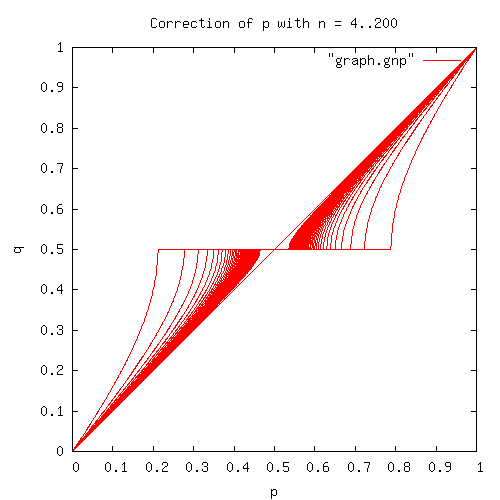
\includegraphics[scale=0.5]{graph.png}
\caption{
For a set of values for \(n\) (with \(n = 2\tilde{n}\)) ranging from \(4\) (farthest on the left and right) to \(200\) (nearest to \(f(p) = p\))}
\end{figure}

\newpage
\section{Code}
Finally we can put our results into a code (\(N = \tilde{n}\)):\\

\begin{verbatim}
if( p < 0.5*(1 - sqrt( (2*N-2) / (2*N-1) )) )
    q = 0.5 * (1 - sqrt( 4*p*(1-p) * (2*N-1) / (2*N-2) ) );
else
if( p > 0.5*(1 + sqrt( (2*N-2) / (2*N-1) )) )
    q = 0.5 * (1 + sqrt( 4*p*(1-p) * (2*N-1) / (2*N-2) ) );
else
    q = 0.5;
\end{verbatim}

or for the general formula with \(n \neq 2\tilde{n}\) (\(M = n, N = \tilde{n}\)):\\
         
\begin{verbatim}
if( p < 0.5 * (1 - sqrt( ((N-1)*M) / ((M-1)*N) ) ) )
    q = 0.5 * (1 - sqrt( 4*p*(1-p) * ((M-1)*N) / ((N-1)*M) ) );
else 
if( p > 0.5 * (1 + sqrt( ((N-1)*M) / ((M-1)*N) ) ) )
    q = 0.5 * (1 + sqrt( 4*p*(1-p) * ((M-1)*N) / ((N-1)*M) ) );
else
    q = 0.5;
\end{verbatim}

The main advantage of this code is that only minimal changes to the code have to be made because this way of reducing the diversity loss is problem independent (at least for bitstrings on a flat landscape in UDMA). The code has to be inserted just after determining the distribution \(p\).


\section{Multiple components}

If we set \(C > 1\), i.e. bitstrings longer than one bit, we will get similar results. While equation \(3\) does use \(C\) to determine the diversity of a generated population we can look at each component seperately as they are not connected in UMDA (in a flat fitness landscape). All bits belonging to one component in the population are created with an own distribution \(p\) that is independent from the other \(p\). Therefor we can handle a problem with \(C > 1\) like \(C\) seperate problems, each with one component.
How interconnected components would affect the diversity is out of the scope of this paper and remains to be investigated.


\newpage
\section{Tests}

\subsection{General test configuration}

For both tests, OneMax and Flat fitness landscape, 50 seperate were repeatedly (with varying parameters) made.\\
6 different algorithms were tested:

\begin{itemize}
\item {\bf No correction}: The new distribution \(p\) for each component is simply calculated by dividing the number of 1's by the sample size
\item {\bf No correction + bounded}: Same as (1) but in the case \(p\) gets above \(1 - \frac{1}{\tilde{n}}\) or below \(\frac{1}{\tilde{n}}\) it is corrected to these boundaries
\item {\bf Laplace correction}: The new \(p\) is calculated by \(\frac{k + 1}{\tilde{n} + 2}\)
\item {\bf Corrected distribution}: Same as (1), but the resulting \(p\) is corrected with the formula discussed in the previous section
\item {\bf Corrected distribution + bounded}: Same as (2) but with the correction of \(p\) before checking the boundaries
\item {\bf Corrected distribution + Laplace}: Same as (3) but with the correction of \(p\) afterwards
\end{itemize}

Using the for each component newly calculated distribution \(p\) we generate the new population of the size \(n\) depending on our parameter called 'Exact Random Distribution'. If it is not set we create each member of the population individually, if it is set we distribute \(pn\) '1' and \((1-p)n\) '0' between the individuals.\\
Tests have shown that the variance of the runs themselves are of no significance so it is are not included in the graphs.\\
The graphs were created with the help of gnuplot and C++, the actual program will be availble with a later version of this paper on CD-ROM.\\

\subsection{Flat fitness landscape}

In this test we examine the behaviour of the algorithms in terms of their diversity with varying parameters on a flat fitness landscape. It is basicly a 'needle in a haystack' problem where the needle is not found within the 200 generations, i.e. all solutions have the same fitness. The problem size is a bitstring with length 10, i.e. we have 10 components.\\
The additional graph, '1 - 1/N loss / generation', denotes the theoretical loss of diversity according to \cite{Shapiro}.

\begin{figure}[htp]
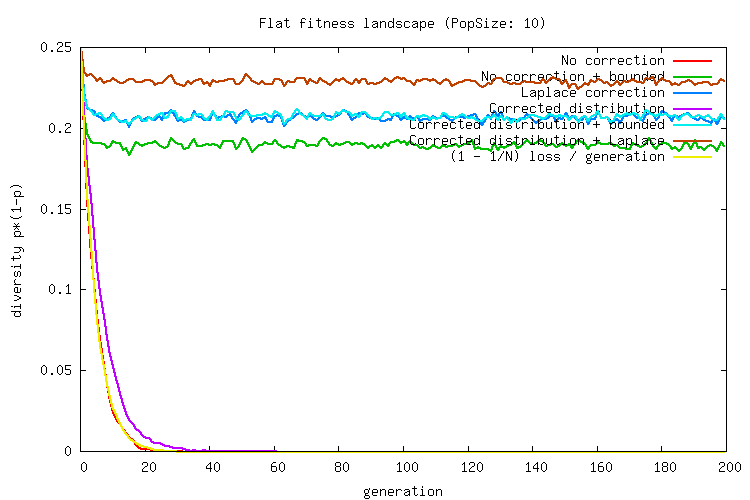
\includegraphics[scale=0.5]{graph_haystack000_diversity.png}
\end{figure}
\begin{figure}[htp]
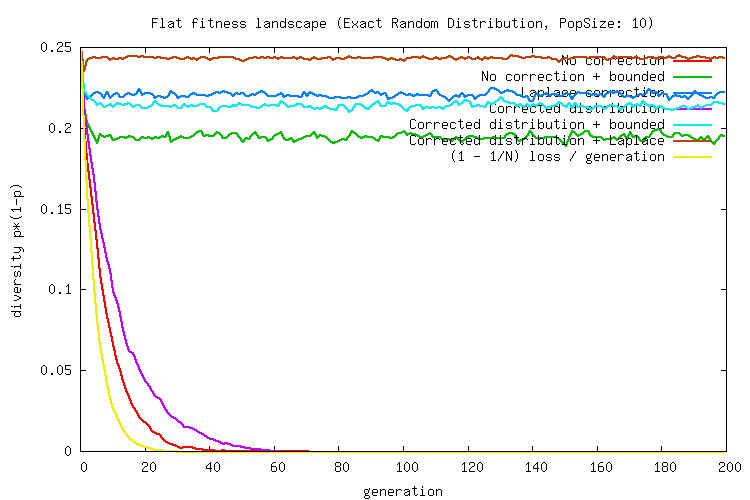
\includegraphics[scale=0.5]{graph_haystack001_diversity.png}
\end{figure}
\begin{figure}[htp]
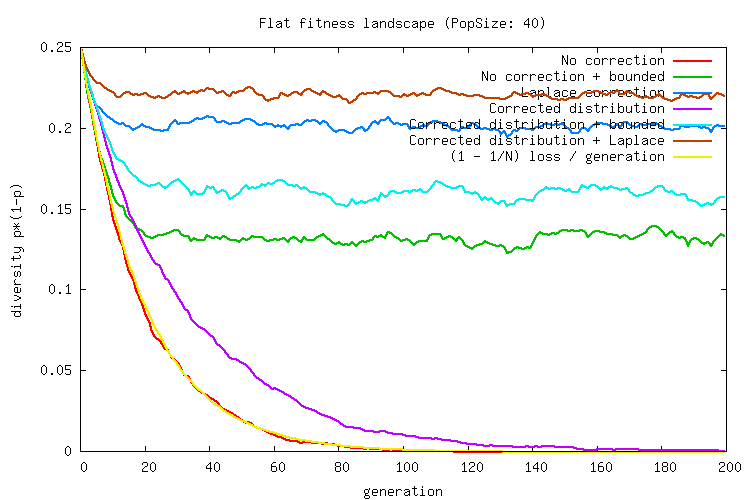
\includegraphics[scale=0.5]{graph_haystack002_diversity.png}
\end{figure}
\begin{figure}[htp]
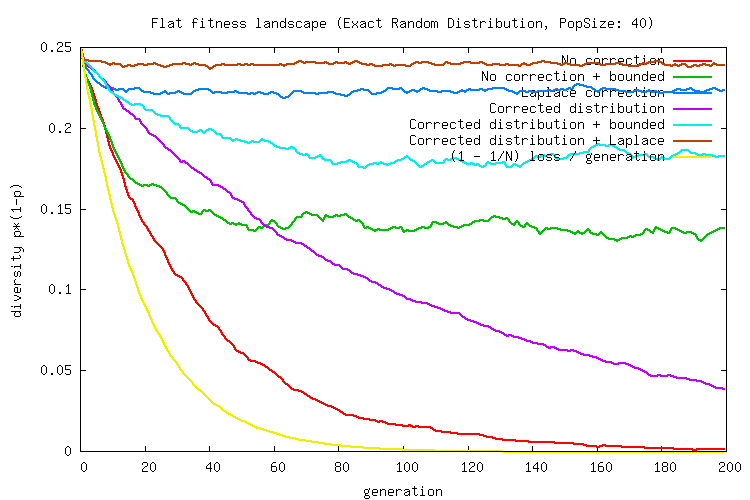
\includegraphics[scale=0.5]{graph_haystack003_diversity.png}
\end{figure}
\begin{figure}[htp]
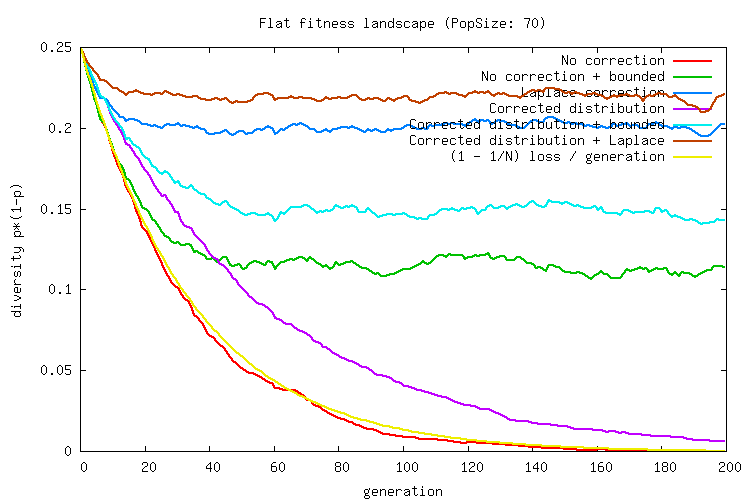
\includegraphics[scale=0.5]{graph_haystack004_diversity.png}
\end{figure}
\begin{figure}[htp]
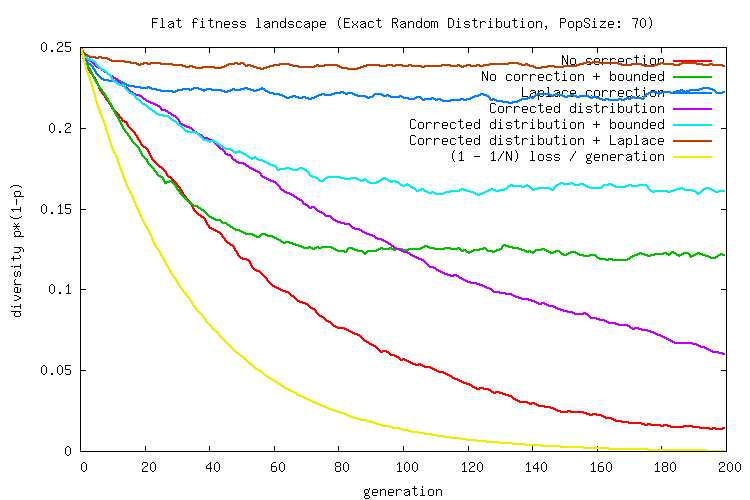
\includegraphics[scale=0.5]{graph_haystack005_diversity.png}
\end{figure}
\begin{figure}[htp]
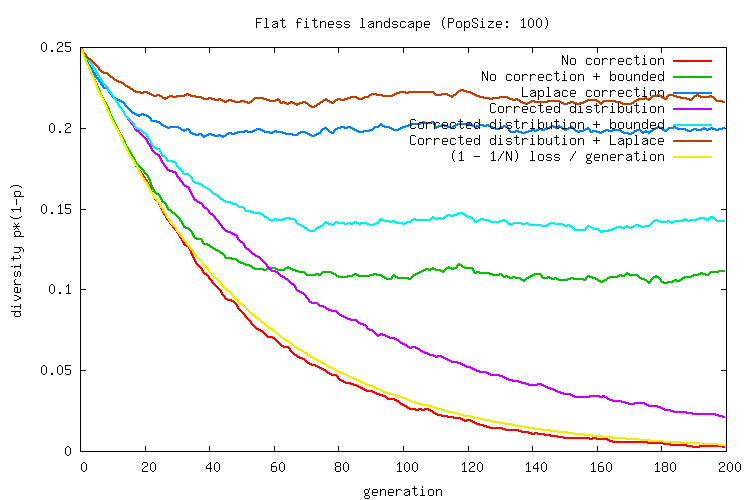
\includegraphics[scale=0.5]{graph_haystack006_diversity.png}
\end{figure}
\begin{figure}[htp]
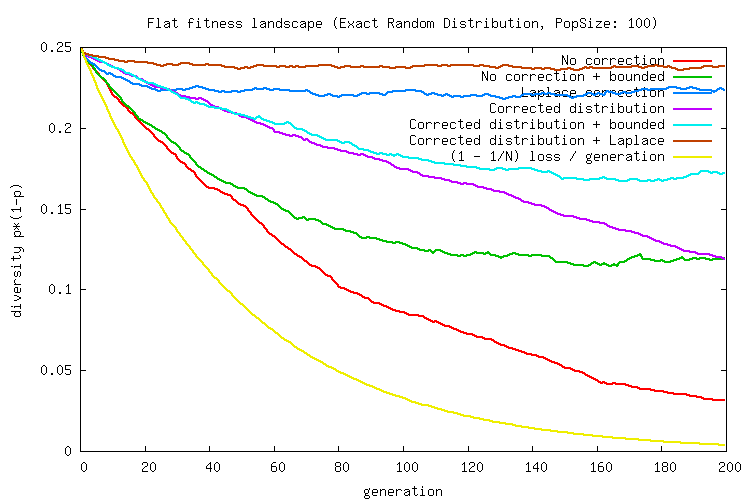
\includegraphics[scale=0.5]{graph_haystack007_diversity.png}
\end{figure}

\newpage
\subsection{OneMax problem}

In this test we examine the behaviour of the algorithms in terms of their fitness with varying parameters with the problem OneMax. The goal is to find the string '111\dots', each '1' in a component of an individual gets rewarded by one fitness point. In our test the problem size if 500.\\
For each generation only the highest fitness of each population is taken into account. Again the graph shows the average of the fitness values of all runs.\\

\begin{figure}[htp]
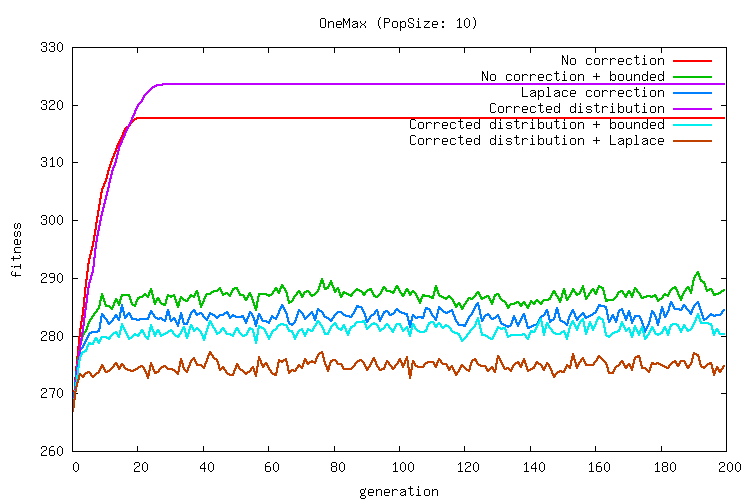
\includegraphics[scale=0.5]{graph_onemax000_fitness.png}
\end{figure}
\begin{figure}[htp]
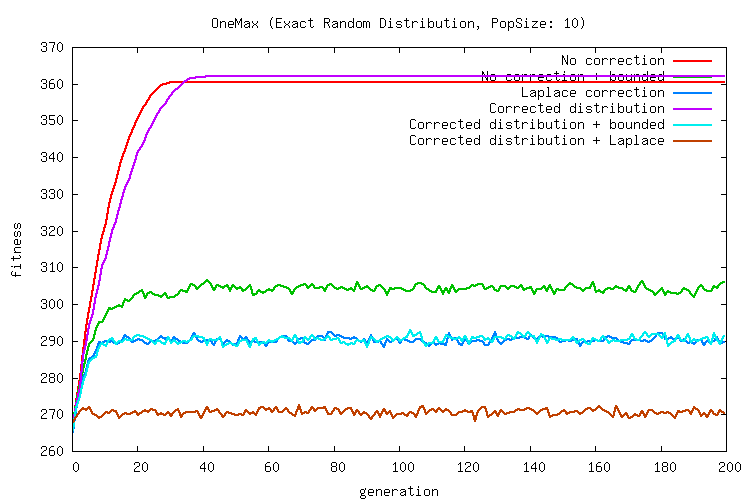
\includegraphics[scale=0.5]{graph_onemax001_fitness.png}
\end{figure}
\begin{figure}[htp]
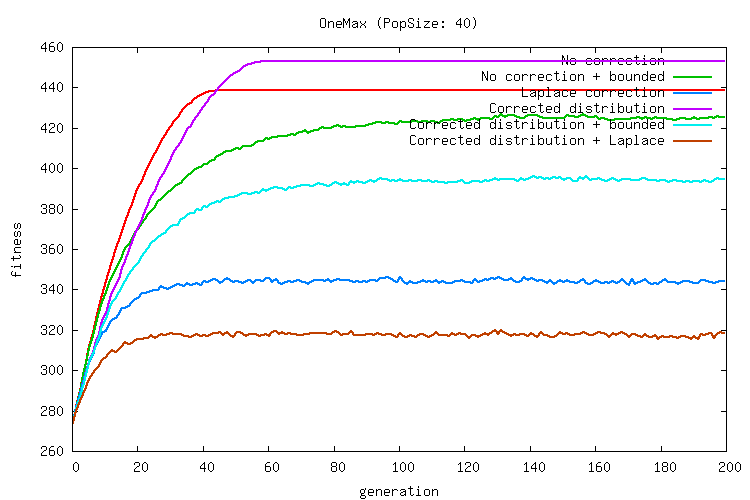
\includegraphics[scale=0.5]{graph_onemax002_fitness.png}
\end{figure}
\begin{figure}[htp]
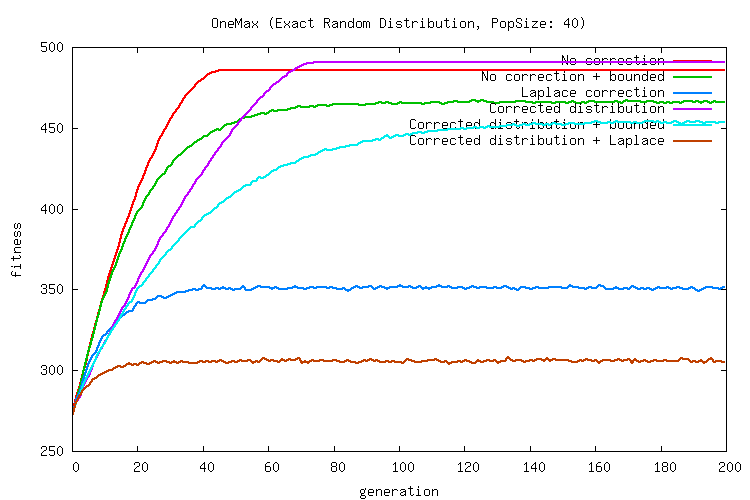
\includegraphics[scale=0.5]{graph_onemax003_fitness.png}
\end{figure}
\begin{figure}[htp]
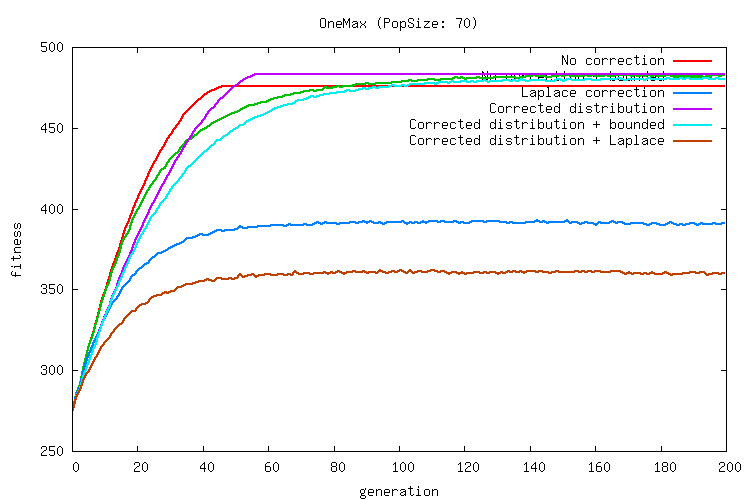
\includegraphics[scale=0.5]{graph_onemax004_fitness.png}
\end{figure}
\begin{figure}[htp]
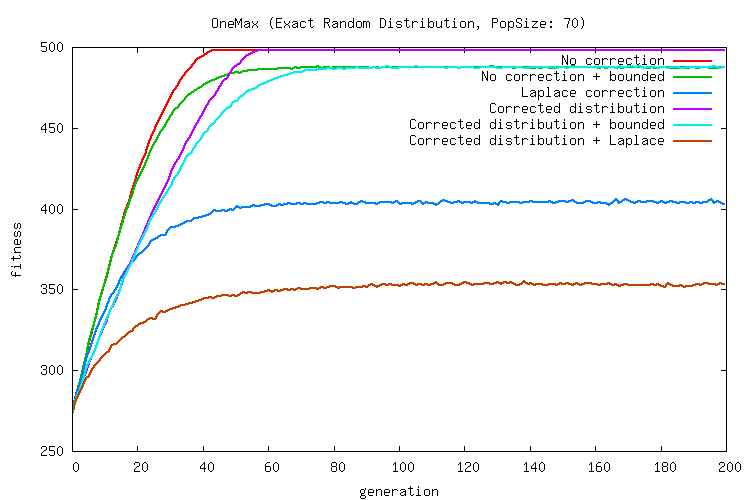
\includegraphics[scale=0.5]{graph_onemax005_fitness.png}
\end{figure}
\begin{figure}[htp]
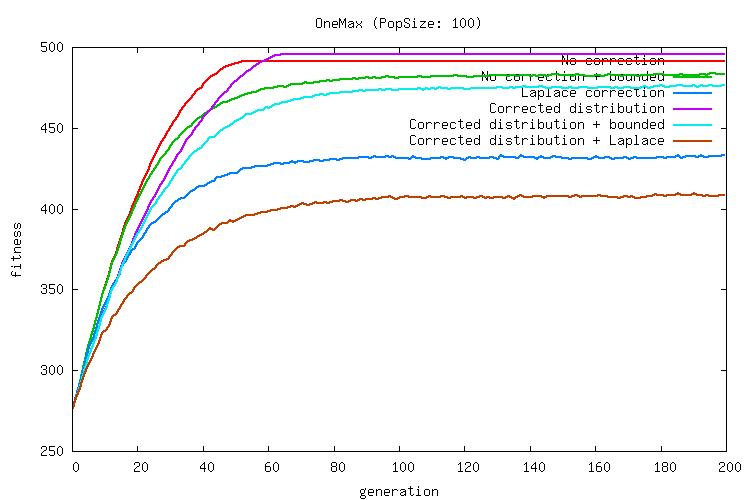
\includegraphics[scale=0.5]{graph_onemax006_fitness.png}
\end{figure}
\begin{figure}[htp]
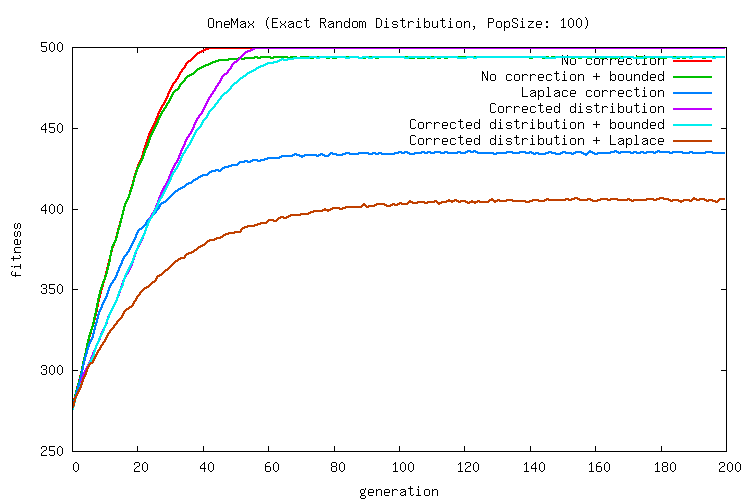
\includegraphics[scale=0.5]{graph_onemax007_fitness.png}
\end{figure}



\newpage
\section{Conclusions}

\subsection{Flat fitness landscape}

With the tests we have shown that our 'Corrected distribution' algorithm does significantly reduce the diversity loss compared to an algorithm with no correction. Making sure that the algorithm does not stall in a component with \(p < \frac{1}{\tilde{n}}\) or \(p > 1 - \frac{1}{\tilde{n}}\) ("bounded") makes sure that the diversity does not drop to zero in the long run. 'Corrected distribution' does not outperform 'Laplace correction' as the latter always corrects any distribution towards \(p = 0.5\).

\subsection{OneMax}

While the OneMax problem does not represent a problem with a real flat fitness landscape (thus our theoretical base does not apply here), a flat fitness landscape can occur if the variance drops and/or the fitness values are very similar (e.g. 010, 100, 001).\\
'Corrected distribution + Laplace' is clearly worse than 'Laplace correction', the changes made to the distribution \(p\) (that we determined on base of the selected individuals) are too big in order to get useful results. As expected 'Laplace correction' itself does not score well, it converges at a significant lower fitness level.\\
'Exact random distribution' seems to generally improve the convergence of methods using not the 'Laplace correction' while being indifferent or being even worse for the 'Laplace correction' itself.\\
At least for the case of 'OneMax' and the given parameter configuration, 'Corrected distribution' in connection with 'Exact Random Distribution' seems to outperform all other methods.

\section{Fields of further research}

According to \cite{Shapiro} the diversity loss of \(1 - \frac{1}{n}\) is independent of \(|A|\) and is valid for a whole class of so-called SML-EDAs, including UMDA, MIMIC, FDA or BOA. In this paper I have assumed that \(|A| = 2\), i.e. that a component can only take two different values. With values \(|A| > 2\) the proof has to be adapted from equation (5) on, depending on how one creates such a population. It also remains to be investigated how a similar correction of the diversity loss is possible with other methods than UMDA that fall into the category of the SML-EDAs. It is probable that the idea itself, i.e. determining the loss of variance due to sampling and calculating it backwards in order to correct the distribution \(p\), seems to be applicable to many different forms of SML-EDAs or even EDAs in general - assuming one can calculate the actual diversity loss.

\begin{thebibliography}{99}
\bibitem{Shapiro} {\sc Shapiro, J.L.:}  \textit{Diversity loss in general estimation of distribution algorithms}, 2006.
\end{thebibliography}
\end{document}

